\documentclass[11pt,a4paper]{article}
\usepackage[utf8]{inputenc}
\usepackage[english]{babel}
\usepackage[T1]{fontenc}
\usepackage{amsmath}
\usepackage{amsfonts}
\usepackage{amssymb}
\usepackage{graphicx}
\usepackage{array}
\usepackage{multirow}
\usepackage[left=2cm,right=2cm,top=2cm,bottom=2cm]{geometry}
\author{Guillem Tocabens}
\title{First measurements}
\begin{document}

\section{Overall setup}

The global setup uses three detectors: two scintillator detectors, placed on the sides (black squared boxes on the picture, Figure \ref{Setup}) and one semi conductor detector - hyperpure germanium detector - below the collimated source (grey cylinder on the picture). The source is placed on the top lead brick which contains a hole in the middle to collimate the radioactive source. In that position, the source is 97mm from the top of the crystal, which is 5mm from the top of the cryostat (grey cylinder), and collimated in a 5mm hole through an 80mm lead brick. the source is covered by a little lead brick and the setup is shielded by lead to avoid propagation of gamma radiation away from the setup (see Figure \ref{Setup_front}).

\begin{figure}[!h]
\centering
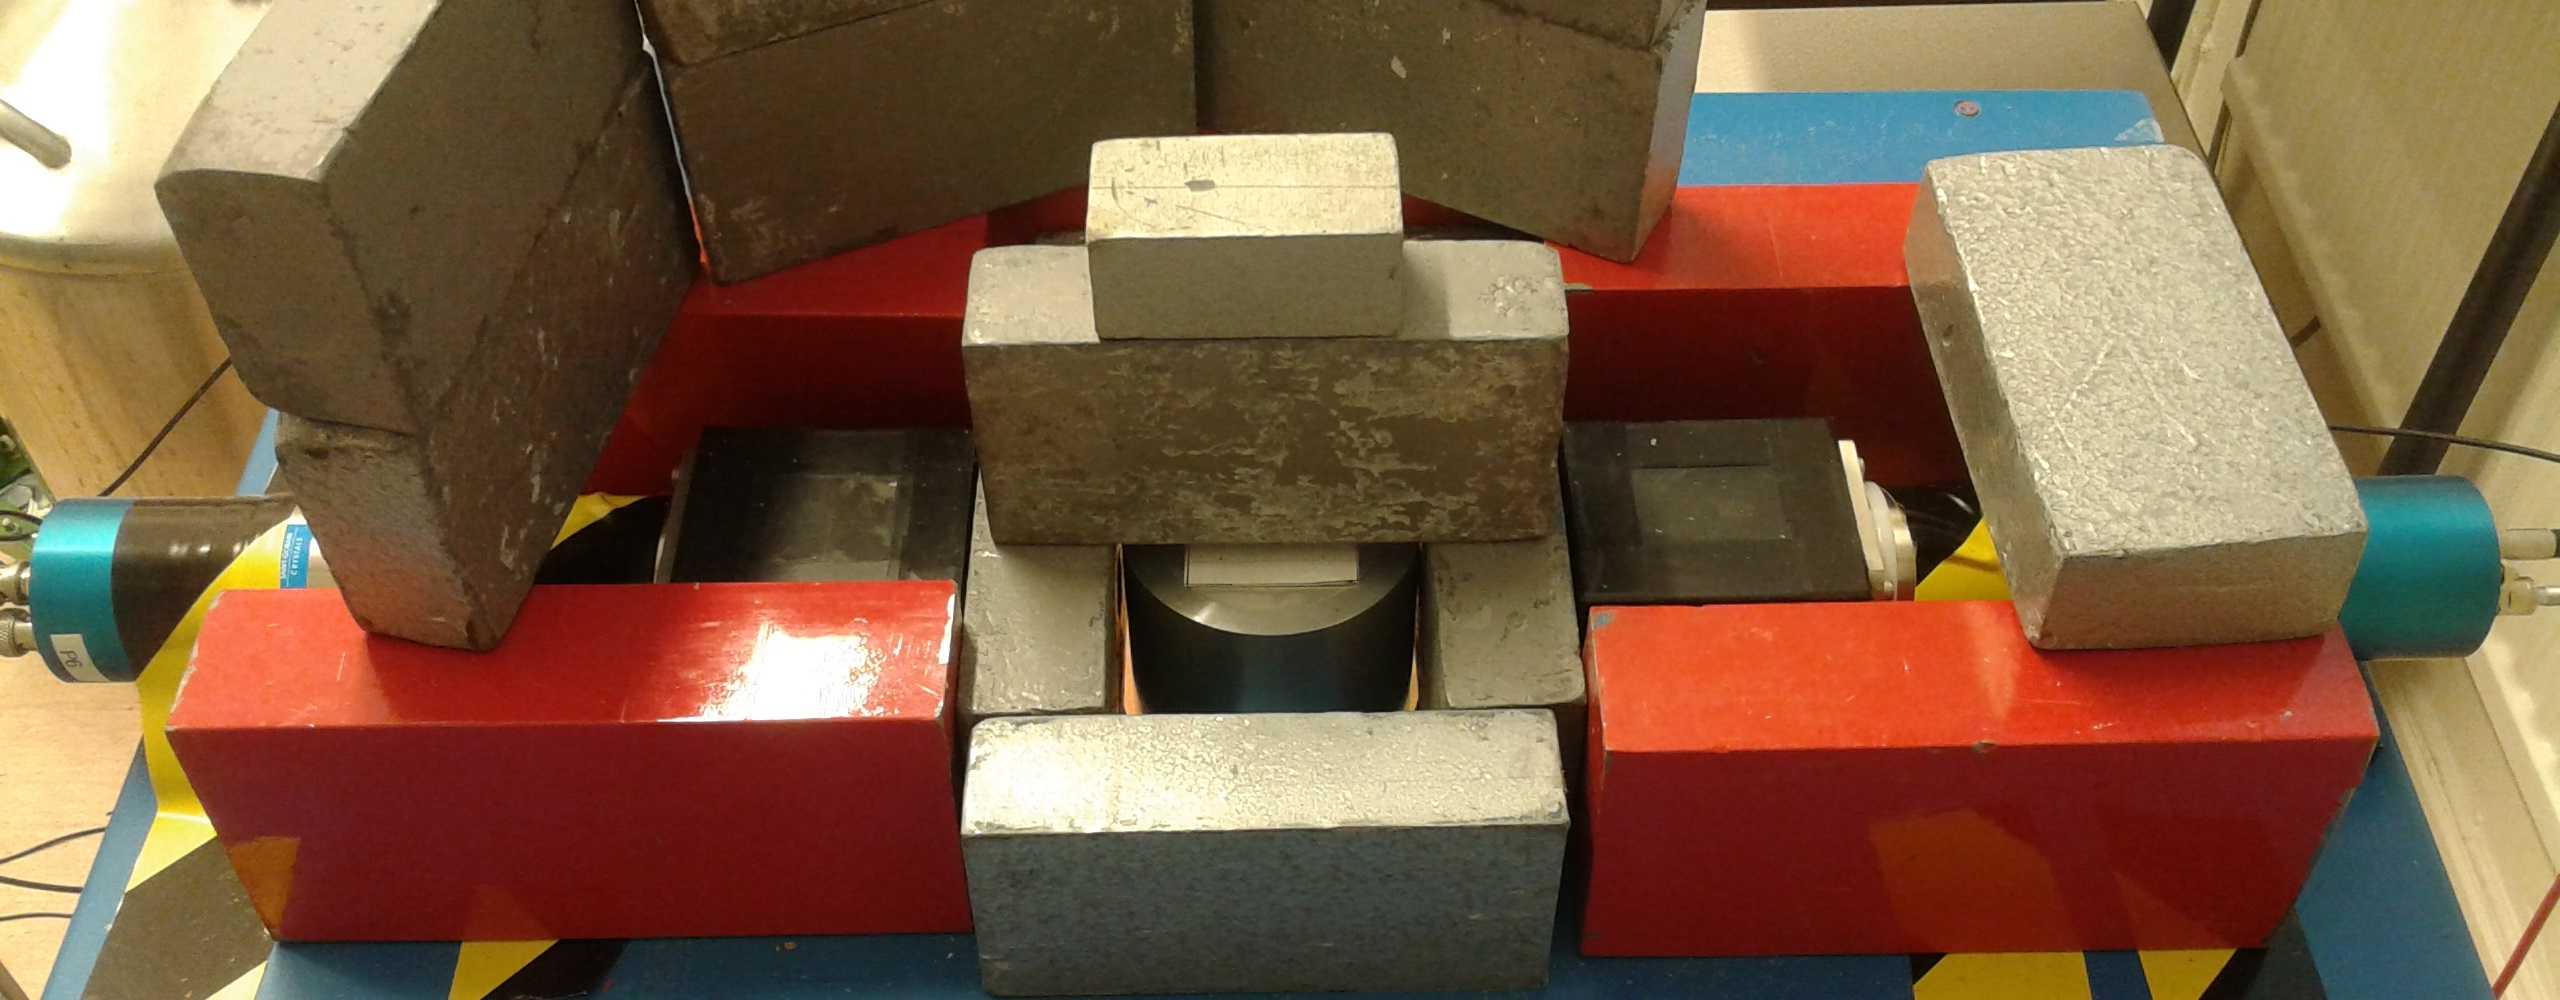
\includegraphics[scale=0.15]{New_setup_back.jpg}
\caption{Back of the original setup. The scintillator detectors are the black squared boxes on the sides of the germanium detector, placed in a cryostat (grey cylinder in the middle).}
\label{Setup}
\end{figure}

\begin{figure}[!h]
\centering
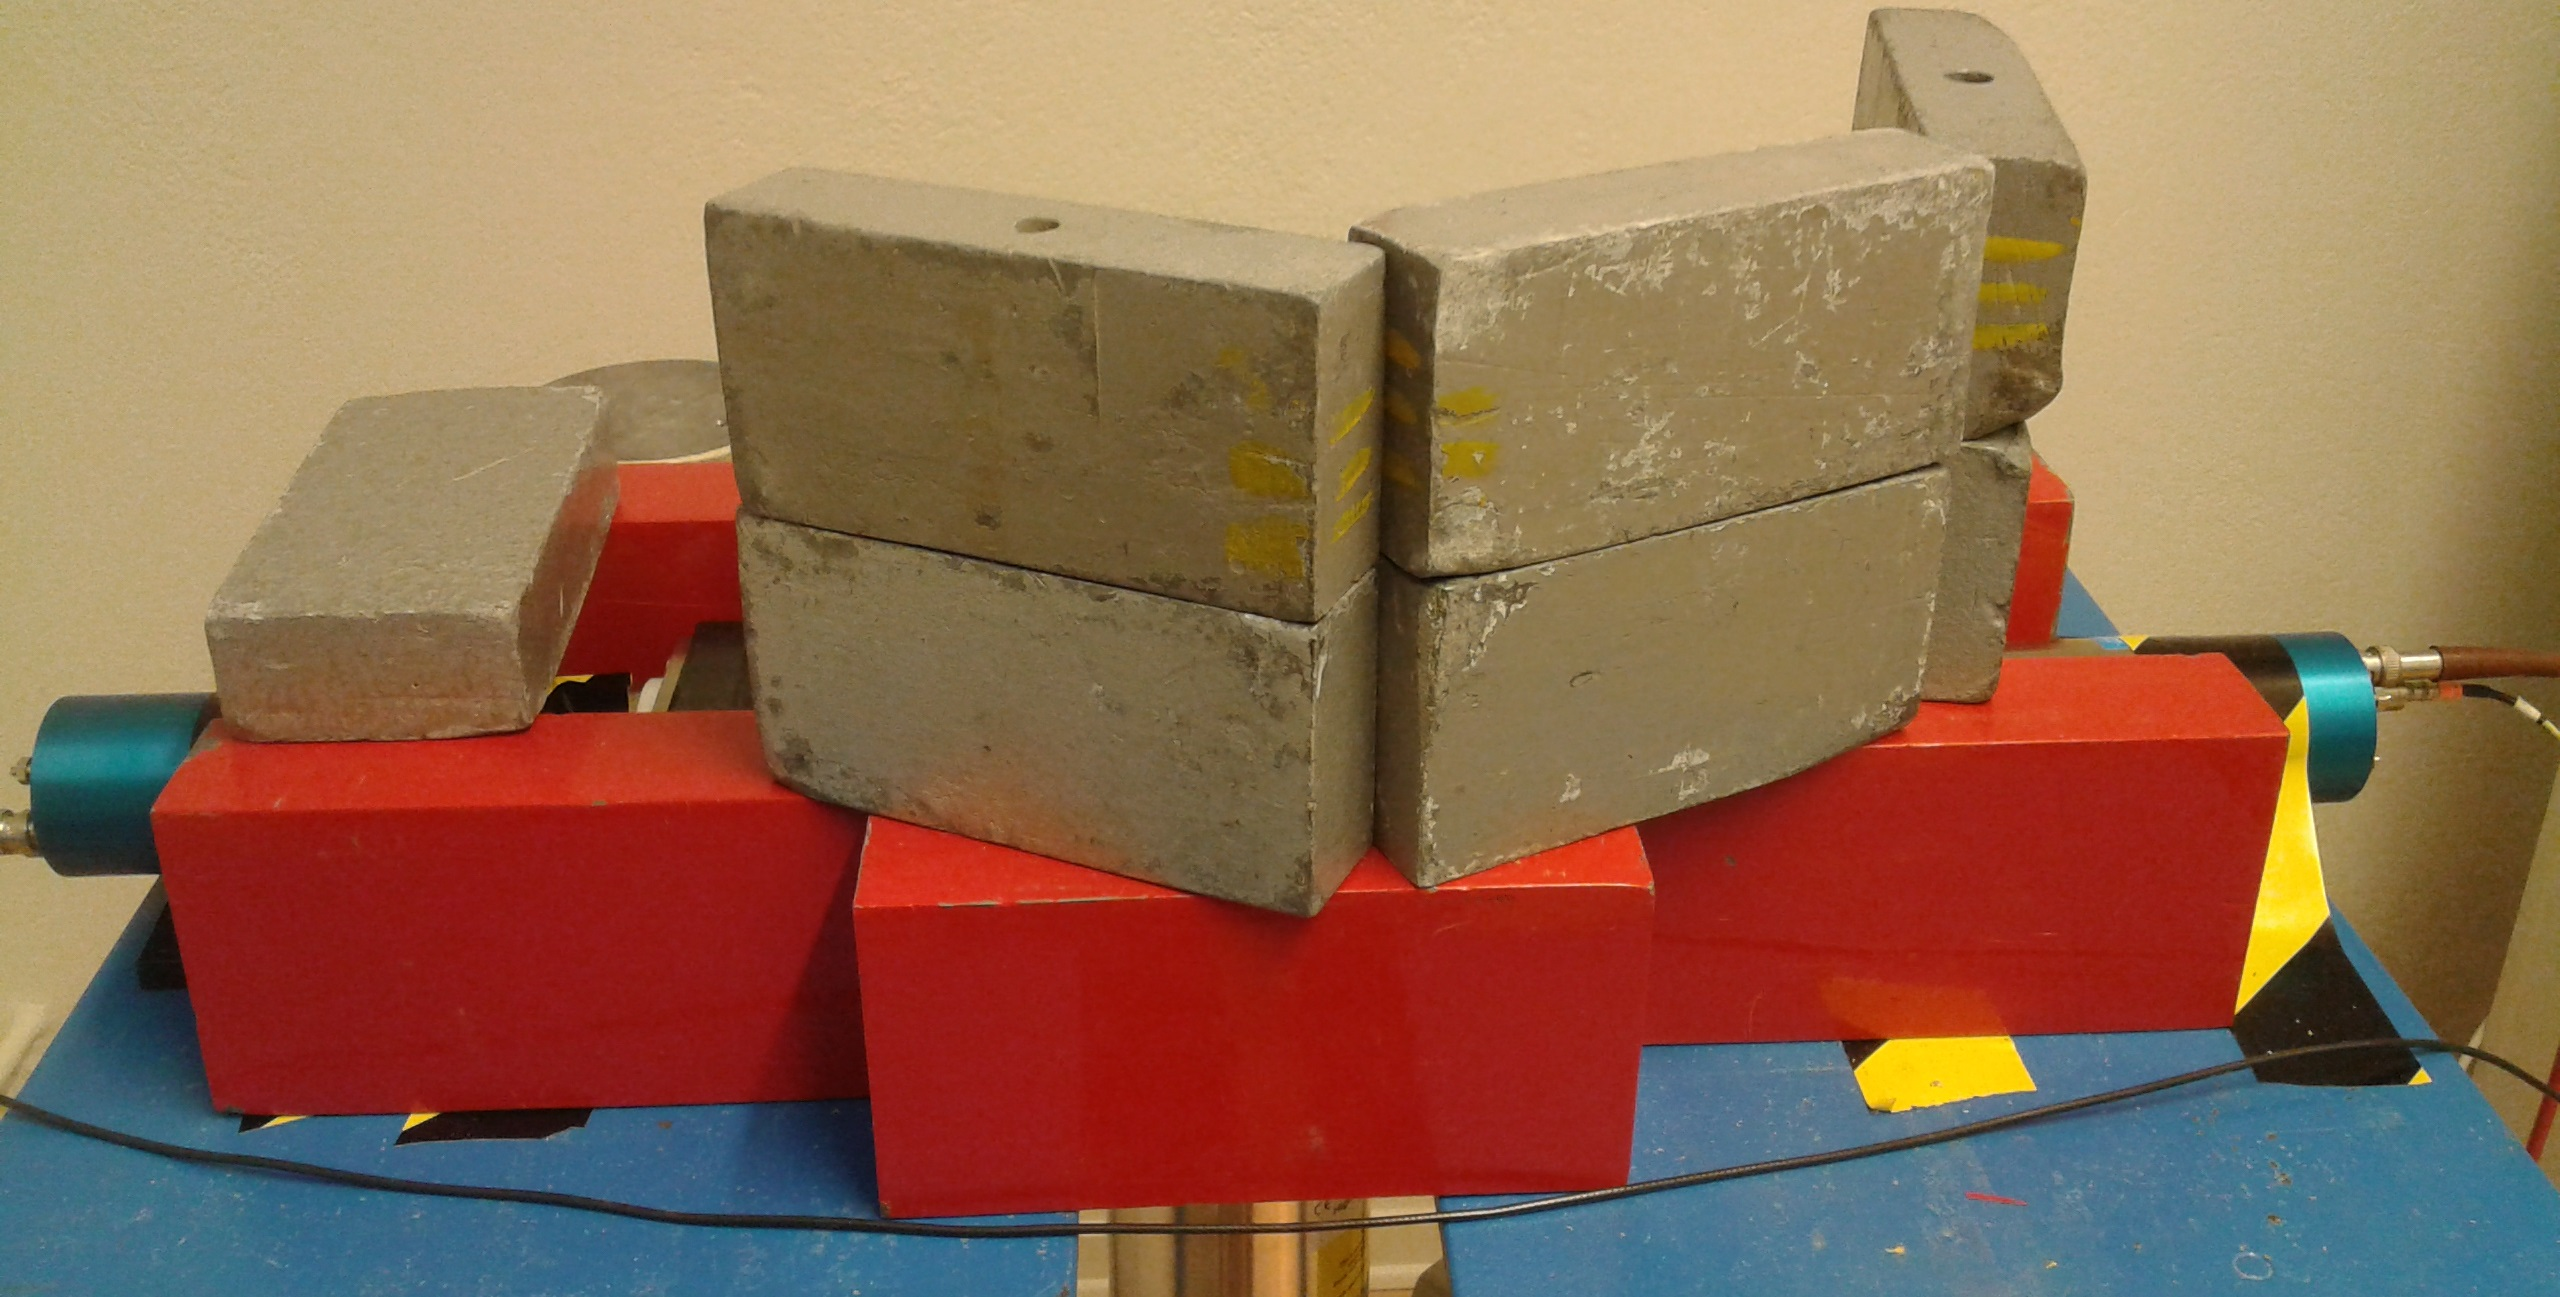
\includegraphics[scale=0.15]{New_setup_front.jpg}
\caption{Front side of the original setup (with the lead shielding).}
\label{Setup_front}
\end{figure}

\section{Scanning the prototype detector}

For this first set of measurements, we did not use the scintillator detectors but only the germanium detector. The goal of this experiment was to determine some properties of the detector depending on the location of the collimated source. Therefore, we collimated the source in five different places on the top of the crystal: one measurement was performed with the collimator in the center of the crystal surface, and four were performed with the collimator in the corners of the crystal surface. The scanning went as described below (see scheme Figure \ref{scan}) and we used two different cobalt sources: one of $^{60}$Co and one of $^{57}$Co (the decay schemes are shown in Figure \ref{decayCos}).

\begin{figure}[!h]
\centering
\includegraphics[scale=0.6]{scan.png}
\label{scan}
\caption{Scheme of the top of the germanium crystal and how it was scanned. Each circle represents a position of the collimated source to which we associate a number (distances are in mm).}
\end{figure}

\begin{figure}[!h]
\centering
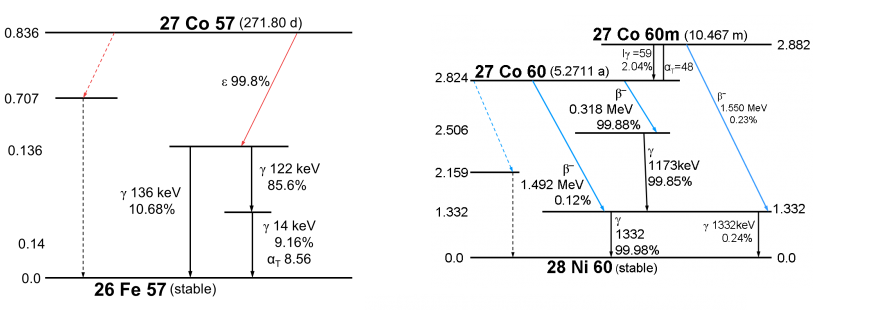
\includegraphics[scale=0.9]{Cos_decays.png}
\label{decayCos}
\caption{Decay schemes of $^{60}$Co and $^{57}$Co.}
\end{figure}

In the case of $^{60}$Co, the source was held in one of the positions until the net area of the studied peak (peak at 1332keV) contained at least 100~000 counts. The $^{57}$Co source being way less active, the measurement was stoped when the net area of the studied peak (peak at 122keV) contained around 1~000 counts.

\end{document}